% Chapter 2

\chapter{Marco Teórico} % Main chapter title

\label{Chap:Marco} % For referencing the chapter elsewhere, use \ref{Chapter2} 

%----------------------------------------------------------------------------------------

% Define some commands to keep the formatting separated from the content 
%\newcommand{\keyword}[1]{\textbf{#1}}
%\newcommand{\tabhead}[1]{\textbf{#1}}
%\newcommand{\code}[1]{\texttt{#1}}
%\newcommand{\file}[1]{\texttt{\bfseries#1}}
%\newcommand{\option}[1]{\texttt{\itshape#1}}

%----------------------------------------------------------------------------------------

\section{Introducción}

En esta sección se presenta la teoría de varios elementos clave en el prototipo a utilizar. Partiendo desde la definición de GPS, pasando por una breve historia, su fundamento matemático y las causas de error en las mediciones, hasta el software utilizado y los dispositivos específicos utilizados en este trabajo, se presentan datos de funcionamiento y su relación con el proyecto.

\section{El sistema de Posicionamiento Global - GPS}

\begin{figure}[ht]
\centering
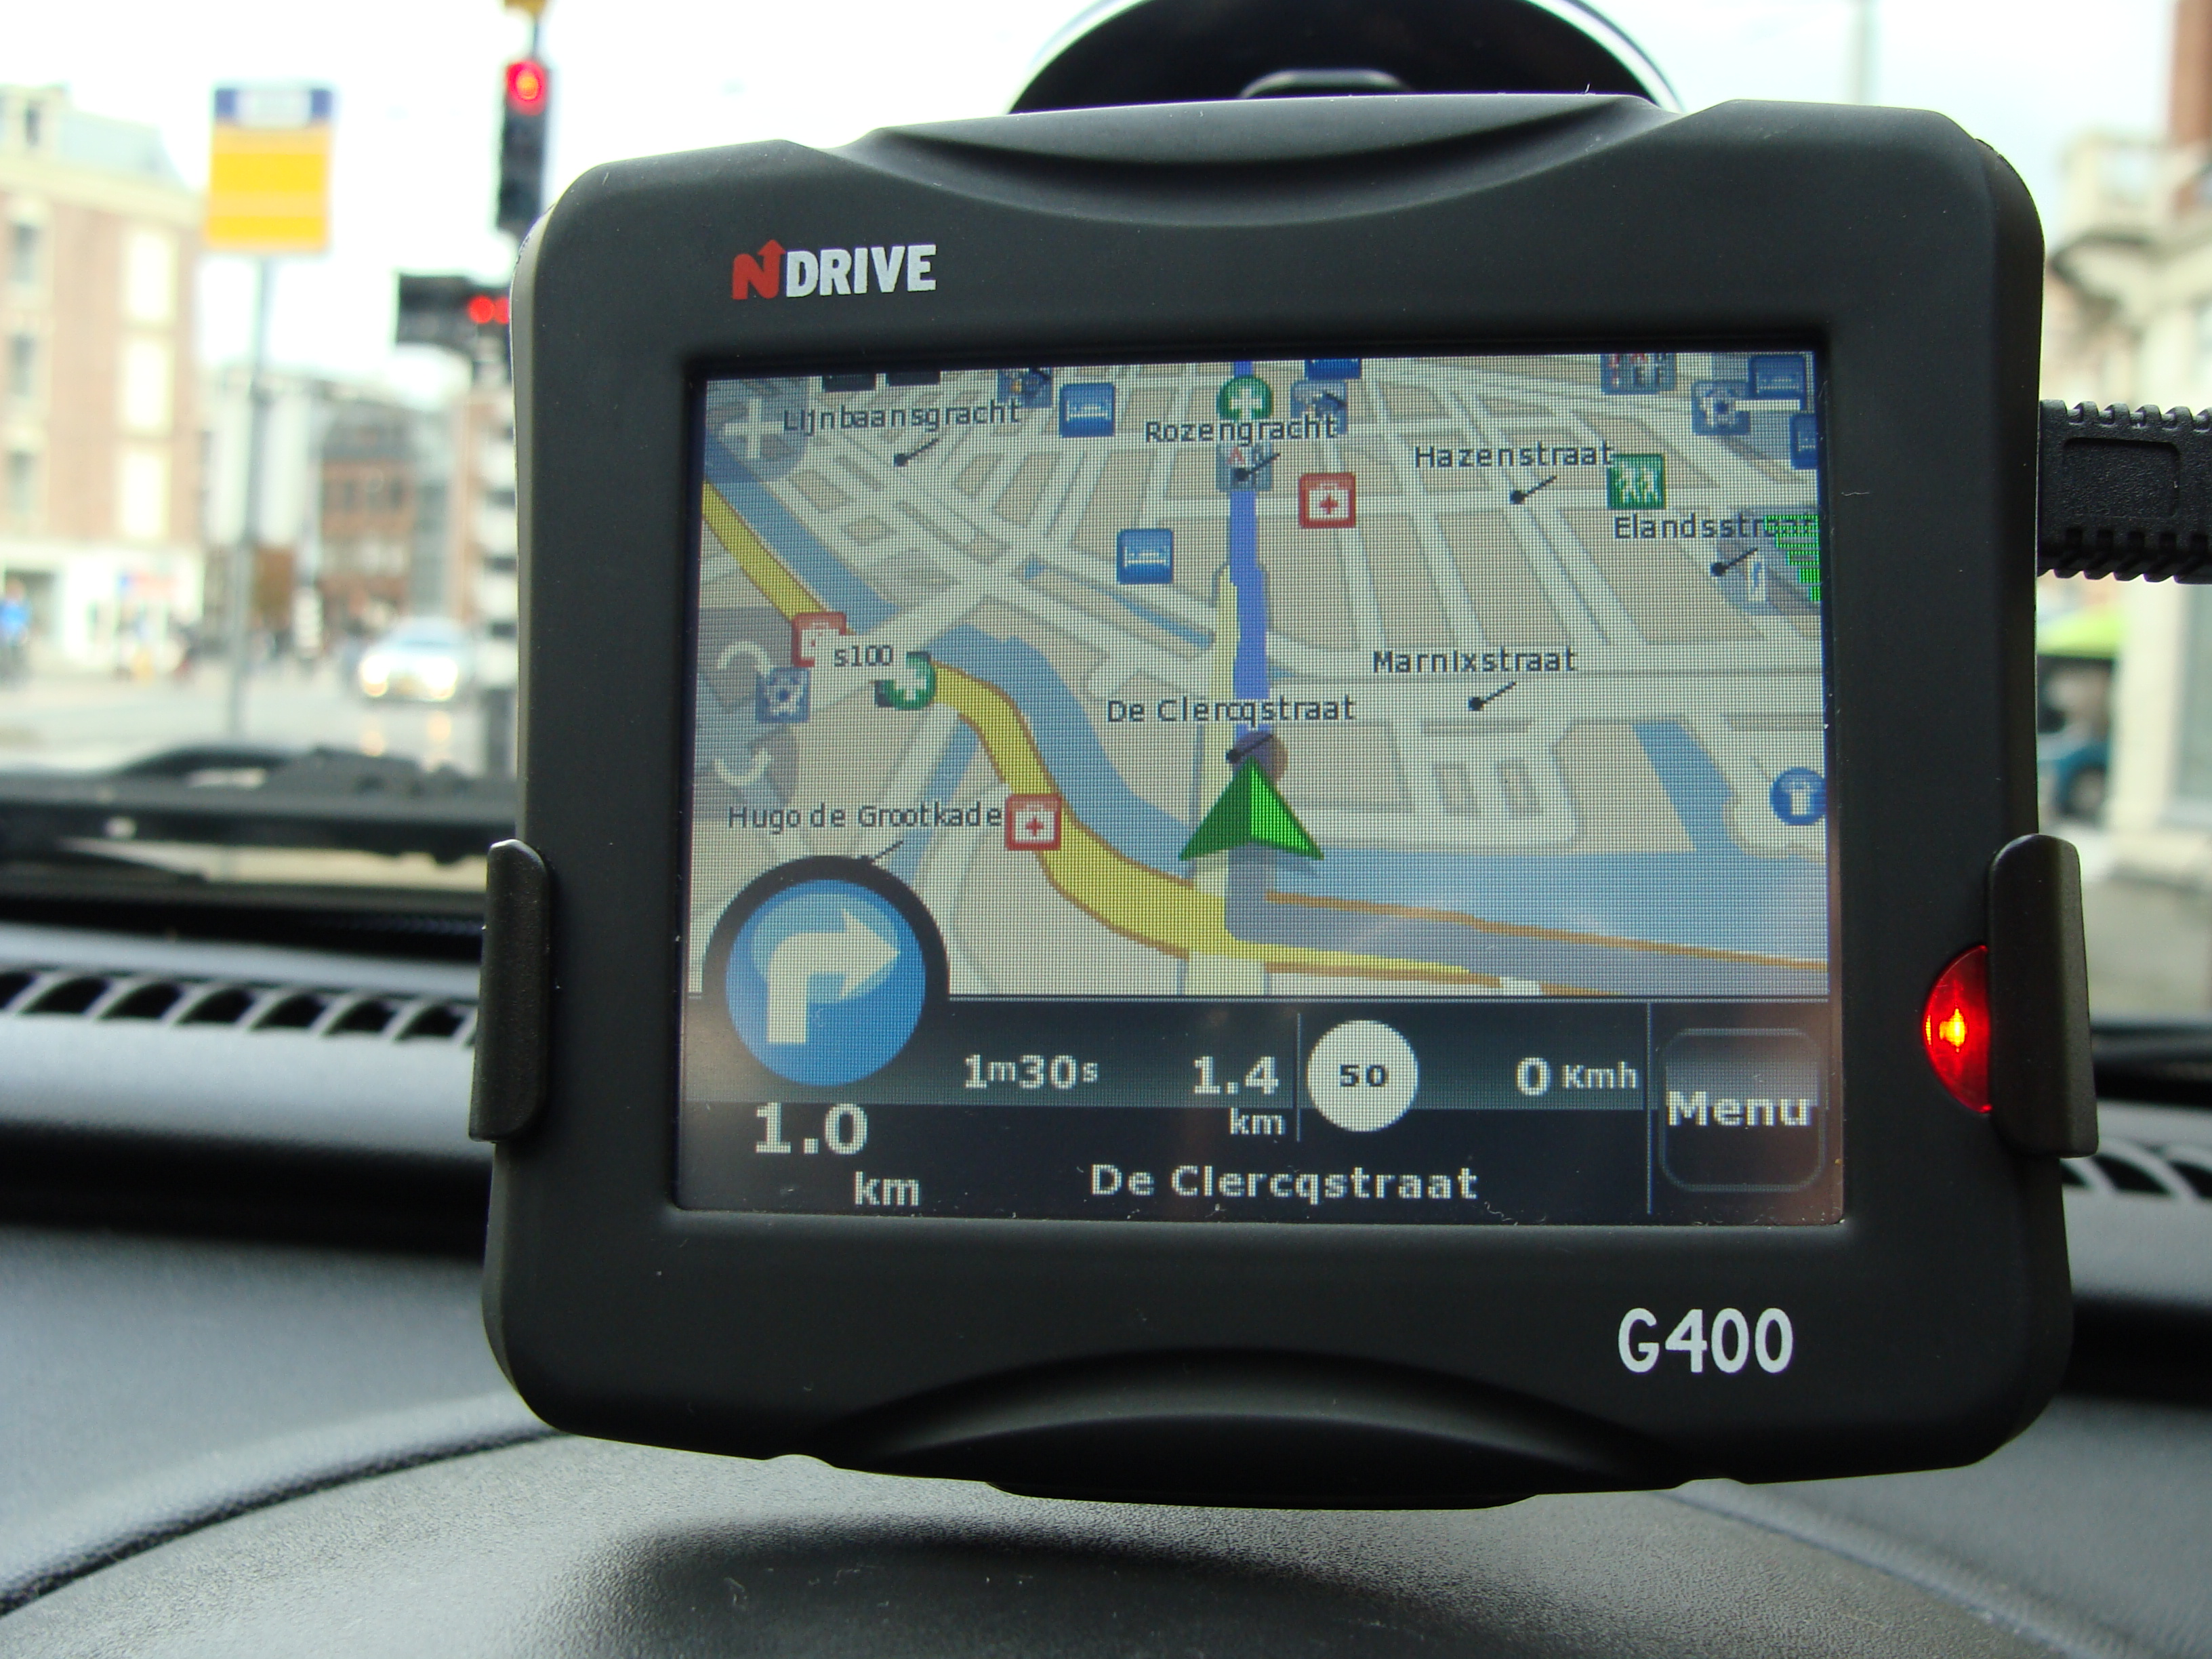
\includegraphics[scale=0.07]{Figures/GPS}
\caption[Sistema de Posicionamiento Global.]{Sistema de Posicionamiento Global.\footnotemark}
\label{fig:GPS}
\end{figure}

\footnotetext{Imagen tomada de: \href{https://upload.wikimedia.org/wikipedia/commons/thumb/9/9f/NDrive_GPS.jpg/1280px-NDrive_GPS.jpg}{https://upload.wikimedia.org/}}

GPS fue iniciado en 1973 para su uso con fines militares por los Estados Unidos de Norteamérica. Su objetivo principal es la determinación de las coordenadas espaciales bajo una referencia mundial. Para dichos propósitos, se necesita una recepción de señales de un mínimo de cuatro satélites, cuyas coordenadas son plenamente conocidas \cite{huerta2005gps}.

\subsection{Historia}

\subsubsection{Antecedentes}
Antes de que GPS funcionara mediante satélites, ya estaban implementados varios sistemas de localización radio-terrestres. Uno de ellos era conocido como LORAN (\textit{Long Range Navigation}, Navegación de largo alcance por sus siglas en inglés). Se fundamentaba por el envío de una señal desde distintos emisores. Al percibir señal de tres distintos emisores, podía determinar su posición. \\

Fue tras el lanzamiento del Sputnik\footnotemark, que investigadores norteamericanos descubrieron que era posible la determinación de la posición gracias a la deformación de una señal por efecto Doppler. Así, si era posible conocer la posición del satélite conociendo la posición del observador en la Tierra, a la inversa, sería posible conocer la posición de un observador conociendo la posición del satélite.

\footnotetext{Satélite ruso, el primero de la historia.}

\subsubsection{Con satélites en órbita}
El primer sistema que utilizaba la triangulación mediante satélites fue \textit{TRANSIT} en 1960, entrando en operaciones hasta 1965. Constaba de seis satélites en seis planos, contando con cobertura mundial. \\

Requería que el observador realizara un seguimiento de 15 minutos a la constelación satelital, pudiendo acceder a ellos cada hora y media. Su error de precisión rondaba los 250 metros.\\

En 1973 se propuso el \textit{DNSS} (Defense Navigation Satellite System, Sistema de Navegación Satelital de Defensa por sus siglas en inglés), cambiando de nombre a \textit{NAVSTAR} (Navigation System Time and Ranging, Sistema de Navegación por Tiempo y Distancia, por sus siglas en inglés), después a \textit{NAVSTAR-GPS} y finalmente a \textit{GPS} \cite{termal2014prototipo}.

\subsection{La constelación NAVSTAR}

\begin{figure}[ht]
\centering
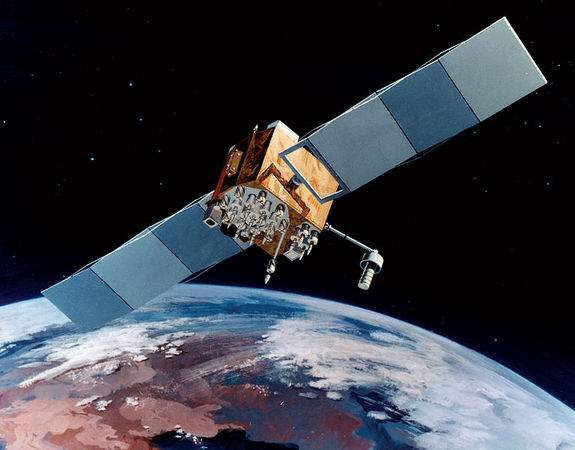
\includegraphics[scale=0.29]{Figures/Navstar}
\caption[Satélite de la constelación NAVSTAR.]{Satélite de la constelación NAVSTAR\footnotemark.}
\label{fig:NAV}
\end{figure}

\footnotetext{Imagen tomada de: \href{https://upload.wikimedia.org/wikipedia/commons/thumb/f/f4/Navstar-2F.jpg/613px-Navstar-2F.jpg}{https://upload.wikimedia.org/}}

La constelación \textit{NAVSTAR} está conformada por los satélites que se utilizan para triangular la posición. Se propuso que fueran 24 satélites situados en seis planos de cuatro satélites cada uno, con cobertura en toda la Tierra. \\

La constelación ha sido lanzada en conjuntos llamados \textit{Blocks} (bloques en inglés), distribuidos de la siguiente manera.

\begin{itemize}
	\item Block I (1978 - 1985): 11 satélites lanzados, \textcolor{blue}{10 puestos en órbita con éxito}.
	\item Block II (1989 - 1990): \textcolor{blue}{9 satélites puestos en órbita con éxito}.
	\item Block IIA (1990 - 1997): \textcolor{blue}{19 satélites lanzados con éxito}.
	\item Block IIR (1997 - 2004): 11 satélites lanzados, \textcolor{blue}{12 satélites lanzados con éxito}.
	\item Block IIR-M (2005 - 2009): \textcolor{blue}{8 satélites lanzados con éxito}.
	\item Block IIF (2010): \textcolor{blue}{1 satélite lanzado con éxito} \citep{termal2014prototipo}
\end{itemize}

\subsection{Estructura}

GPS está conformado por tres segmentos:

\begin{itemize}
	\item Segmento espacial: los satélites.
	\item Segmento de control: estaciones terrestres.
	\item Segmento de usuario: los receptores.
\end{itemize}
	
\subsubsection{Segmento espacial}

Se conoce como segmento espacial al sistema de satélites que orbitan al planeta Tierra, emitiendo señales que permiten al receptor calcular su posición en el marco de referencia terrestre. \\

Se reparten en seis órbitas sincronizadas y se desplazan a una altitud de 20'000 Km. Cada uno de ellos dan una vuelta a la Tierra en 12 horas. \\

Los satélites son ajustados mediante mensajes NAV enviados desde el segmento de control.

\subsubsection{Segmento de control}

Conjunto de sistemas instalados en la Tierra que permiten el funcionamiento óptimo del segmento espacial.

Conformada por 12 estaciones, de las cuales la principal \textit{MCS} (Master Control Station, Estación de Control Principal por sus siglas en inglés) se encuentra en Colorado, en la Base Schriever de la Fuerza Aérea.	

Tras el envío de nueva información, cada satélite sincroniza su reloj atómico y ajusta las efemérides de su órbita. El cálculo de esta última es a través de un filtro de Kalman, permitiendo una estimación precisa a pesar de múltiples factores externos.

\subsubsection{Segmento de usuario}

Conformado por equipos receptores diseñados para recibir, decodificar y procesar las señales de los satélites. Los parámetros para controlar la calidad de los receptores utilizados son los siguientes:

\begin{itemize}
	\item La antena debe estar bajo cielo abierto recibiendo la señal de los satélites con suficiente potencia.
	\item El reloj interno del receptor debe mantener la sincronización entre receptor y satélites.
	\item El número de canales debe habilitar al receptor para sintonizar un número suficiente de señales.
	\item El procesador debe tener una frecuencia tal que garantice un cálculo correcto de la posición a partir de las señales captadas \cite{termal2014prototipo}.	
\end{itemize}

El segmento espacial y el segmento de usuario están conectadas por dos frecuencias inalámbricas: \textbf{L1} y \textbf{L2}. La primera es de 1575.42 MHz y la segunda de 1227.60 MHz\cite{farrell2008aided}.

\subsection{Dispositivos GPS}
Los dispositivos GPS son aparatos receptores que obtienen la información de los satélites y realizan un procesamiento del mismo para ubicarse en el marco de referencia terrestre. \\

Existen GPS de distintos tamaños y marcas.

\begin{table}[!htb]
\begin{center}
\caption{Características del GPS Navspark RAW.}
\begin{tabular}{|l|}
	\hline
	        \ \ \ \ \ \ \ \ \ \ \ \ \ \ \ \ \ \ \ \ \ \ \ \ \ \ \ \ \ \ \ \ \ \ \ \ \ \ \ \ \ \ \ \ \ \ \ \ \ \ \textbf{Navspark RAW GPS} \\
	\hline
	%\begin{figure}[H]%Example image
		\\  \ \ \ \ \ \ \ \ \ \ \ \ \ \ \ \ \ \ \ \ \ \ \ \ \ \ \ \ \ \ \ \ \ \ \ \ \ \ \ \ 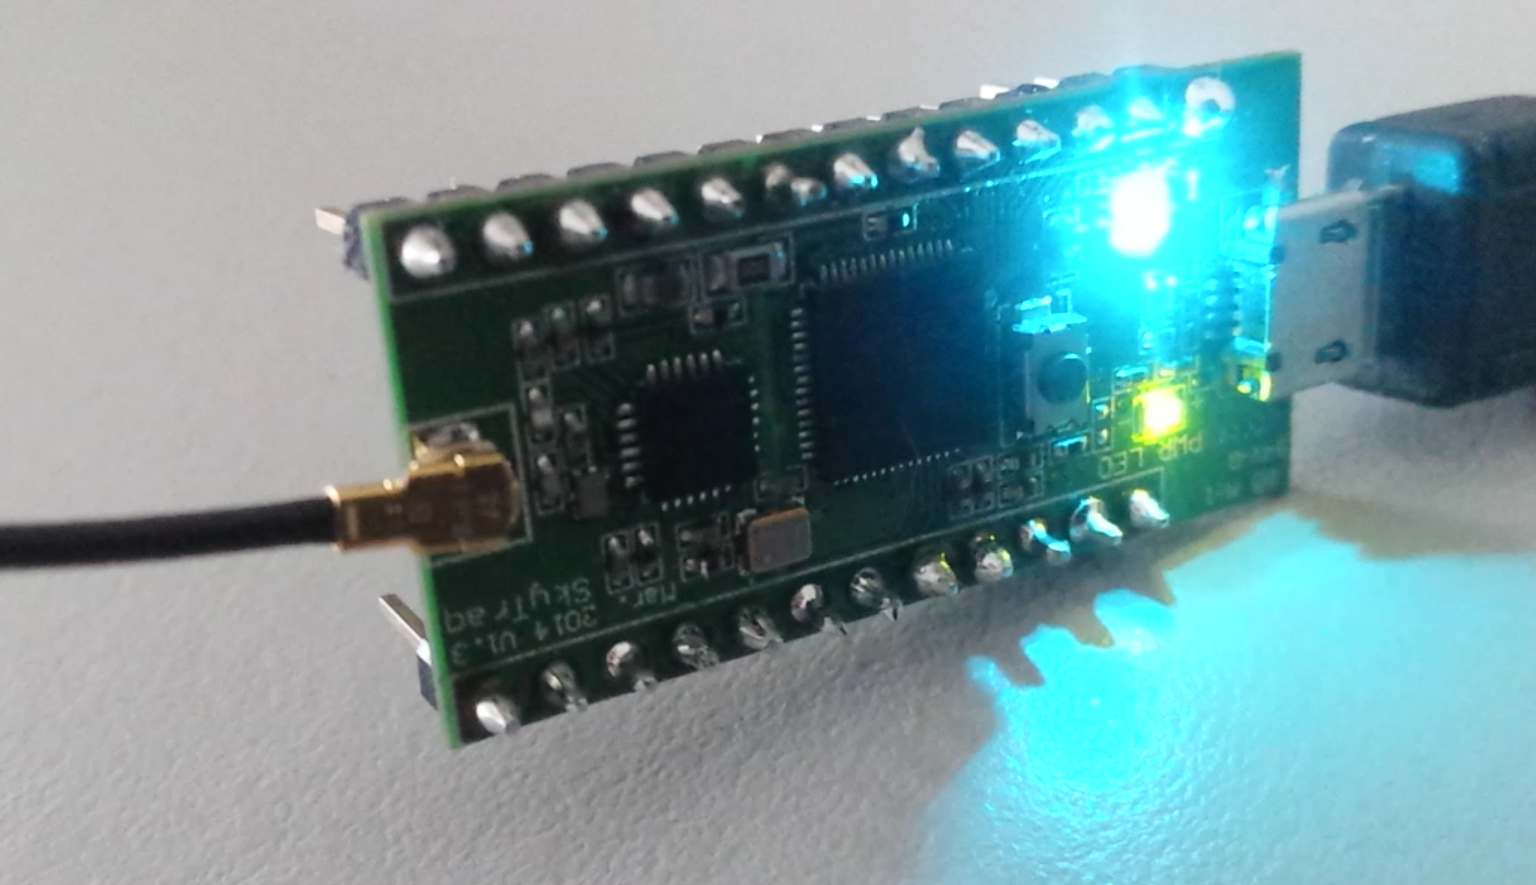
\includegraphics[width=0.37\linewidth]{Figures/NavGPS}
	%	\caption{GPS Navspark.}
		\label{fig:nsraw}\\
	%\end{figure} \\
	
	\textbf{Características:}\\
	%\begin{itemize}
		\tabitem Procesador: 100MHz 32bit LEON3 Sparc-V8 + IEEE-754 Compliant FPU.\\
		\tabitem 17 Digital I/O.\\
		\tabitem GPS con actualización de hasta 20 Hz.\\
		\tabitem Rango de operación: (h $<$ 18000 msnm) \& (v $<$ 515 m/s).\\
		\tabitem Precisión de hasta 2.5 metros.\\
		\tabitem Consumo: 15 ma @ 3.3V \citep{nsraw}.\\
	%\end{itemize} \\
	\hline
\end{tabular}
\end{center}
\end{table}

\begin{table}[!htb]
\begin{center}
\caption{Características del GPS Ublox C94 M8P.}
\begin{tabular}{|l|}
	\hline
	\ \ \ \ \ \ \ \ \ \ \ \ \ \ \ \ \ \ \ \ \ \ \ \ \ \ \ \ \ \ \ \ \ \ \ \ \ \ \ \ \ \ \ \ \ \ \ \ \ \ \ \ \ \ \textbf{Ublox C94 M8P GPS}\\
	\hline
	%\begin{figure}[H] % Example image
	      \ \ \ \ \ \ \ \ \ \ \ \ \ \ \ \ \ \ \ \ \ \ \ \ \ \ \ \ \ \ \ \ \ \ \ \ \ \ \ \ 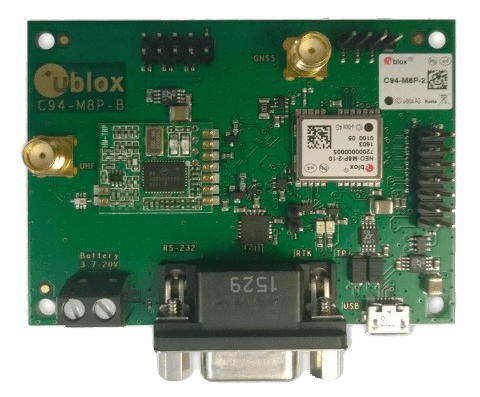
\includegraphics[width=0.25\linewidth]{Figures/ublox}\footnotemark
	%\caption{GPS Ublox. \footnotemark}
	\label{fig:ubx} \\
	%\end{figure} \\
	\textbf{Características: }\\

	%\begin{itemize}
		\tabitem 72 channel u-blox M8 engine GPS L1C/A, GLONASS L1OF, BeiDou B1.\\
		\tabitem GPS con actualizaciones de hasta 10 Hz.\\
		\tabitem Rango de operación: (h $<$ 50000 msnm) \& (v $<$ 500 m/s).\\
		\tabitem Precisión de hasta 2.5 metros.\\
		\tabitem Consumo: 23 ma @ 3.3V.\\
		\tabitem \textcolor{blue}{Incluye módulo de radiofrecuencia.} \citep{ubloxc94}.\\
	%\end{itemize} \\
	\hline
\end{tabular}
\end{center}
\end{table}

\footnotetext{Imagen alojada en www.u-blox.com}

\FloatBarrier

\newpage

\subsection{Principios de funcionamiento}

El objetivo de GPS como sistema de localización es el de calcular la posición de un punto cualquiera en un espacio de coordenadas (x,y,z)\cite{sonnenberg2013radar}, comenzando con el cálculo de las distancias del punto a un mínimo de tres satélites con localización conocida, dicha distancia se obtiene multiplicando el tiempo de propagación de la señal emitida por su velocidad de difusión.\\

Al error de distancias causado por el desfase temporal del reloj del receptor se le llama pseudodistancia \cite{pozo2000sistema}.


\subsection{Fundamento matemático}

A través de las frecuencias L1 y L2, el segmento espacial provee de cobertura a todo el planeta.\\

El objetivo de un receptor GPS en cualquier parte de la Tierra es calcular su posición a través de la determinación de la posición de los satélites que enviaron sus datos de localización en un determinado momento.\\

Los tiempos importantes a utilizar están listados aquí:

\begin{itemize}
\item $t^{'}_r$ - El pseudotiempo en que el receptor toma una medición.\\
\item $t_{sv}$ - El pseudotiempo en el que un satélite emite la señal hacia los receptores.\\
\item $t^{'}_p$ - El pseudotiempo de propagación de la señal emitida por el satélite hasta llegar a la antena del receptor.\\
\item $\Delta t_{sv}$ - El sesgo del reloj satelital.\\
\item $t$ - El tiempo de GPS en el que el satélite emite la señal hacia los receptores.\\
\item $b$ - El sesgo del reloj del receptor.\\
\item $t_r$ - El tiempo de GPS en el que el receptor toma una medición.\\
\item $t_p$ - El tiempo de propagación de la señal desde la antena del satélite hasta la antena del receptor.
\end{itemize}

Las variables $t$ y $t_{sv}$ están dadas por: 

\begin{equation}
\label{Eq:tsv}
t_{sv} = t + \Delta t_{sv}
\end{equation}

Donde $t_{sv}$ es llamado el \textit{tiempo de canal}, porque el receptor mantiene un valor distinto para cada canal.\\

Las variables $t_r$ y $t^{'}_r$ están dadas por:

\begin{equation}
\label{Eq:t_r}
t^{'}_r = t_r + b
\end{equation}

Donde $t^{'}_r$ es el tiempo del receptor y es común para todos los canales. \\

El tiempo de propagación $t_p$ está dado por:

\begin{equation}
\label{Eq:t_p}
t_p = t_r - t
\end{equation}

Los valores típicos para $t_p$ rondan entre 60 ms y 90 ms. \\

Ahora, asumiendo que $b$ inicialmente es desconocida, el cálculo se resume como sigue:\\

\begin{itemize}
\item[1.] En el tiempo $t^{'}_r$, el receptor toma una muestra de todos los canales en los que encuentra señal.\\

\item[2.] En cada canal, el procesador del receptor calcula $t_{sv}$.\\

\item[3.] El procesador del receptor calcula el pseudotiempo de propagación y el pseudorango $\rho$ para cada canal.\\

\begin{equation}
\label{Eq:t'_p}
t^{'}_p = t^{'}_r - t_{sv}
\end{equation}

\begin{equation}
\label{Eq:rho}
\rho = ct^{'}_p
\end{equation}

Donde $c$ es la velocidad de la luz, cuyo valor se muestra en la lista de constantes físicas \ref{Chap:Const}.

\item[4.] Se calcula $\Delta t_{sv}$ utilizando la siguiente ecuación:

\begin{equation}
\label{Eq:Deltat_sv}
\Delta t_{sv}= a_{f0} + a_{f1}(t_{sv}-t_{oc}) + a_{f2}(t_{sv}-t_{oc})^2 + \Delta t_{r}
\end{equation}

Donde $t_{oc}$ y los coeficientes polinomiales son parte del mensaje de navegación proporcionado por los satélites.\\

El término $\Delta t_{r}$ es una corrección relativista:

\begin{equation}
\label{Eq:Deltat_r}
\Delta t_r = FeA^{1/2}sin(E_{k})
\end{equation}

$F$, $e$ y $A$ son constantes definidas en la lista de constantes físicas\ref{Chap:Const}.\\

$E_{k}$ es la ecuación de Kepler de la anomalía de la excentricidad, dada por:

\begin{equation}
\label{Eq:Kepler}
E_k = M_k + esin(E_k)
\end{equation}

Donde $M_k$ es la anomalía media en radianes, dada por: \\

$M_k = M_0 + t_k n$\\

Donde $t_k$ es el tiempo desde la época referenciada, dada por:\\

$t_k = t - t_{oe}$\\

Donde $t_{oe}$ es una constante dada en la observación satelital.\\

$M_0$ es una constante dada en la observación satelital\\

Y $n$ es la media de corrección de movimiento, en radianes por segundo (rps), dada por:\\

$n = n_0 + \Delta n$\\

Donde $n_0$ es la media de compensación de movimiento en rps, dada por:\\

$n_0 = \sqrt{\mu / A^{3}}$\\ 

Y $\Delta n$ es una constante dada por la observación.\\

\item[5.] Partiendo de que es posible calcular $\Delta t_{sv}$ con la ecuación \ref{Eq:Deltat_sv}, se puede calcular $t$ utilizando \ref{Eq:tsv}, de la siguiente manera:

\begin{equation}
\label{t}
t = t_{sv} - \Delta t_{sv}
\end{equation}

Con $t$ calculada, es posible el cálculo de la posición de los satélites. Contando con dichas posiciones y las mediciones de pseudorangos, el receptor puede calcular su propia posición y el sesgo de reloj $b$.

\item[6.] El receptor ahora puede calcular $t_r$ y $t_p$\cite{farrell2008aided}.
\end{itemize}

\subsection{Causas de error}

Como en todo sistema de medición, es probable que un cálculo de una posición se vea afectado por cualquiera de las siguientes: 

\begin{itemize}
	\item Satélites.
	\item Atmósfera.
	\item Rutas múltiples.
	\item Receptor.
\end{itemize} 

\subsubsection{Error causado por el satélite}

\begin{figure}[!ht]
\centering
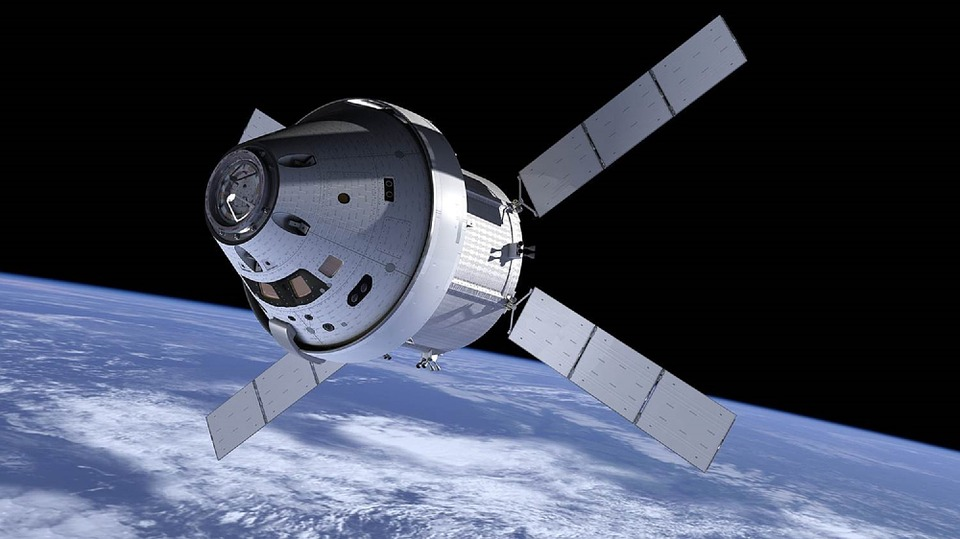
\includegraphics[scale=0.23]{Figures/Sat}
\caption[Error del reloj atómico satelital.]{Error del reloj atómico satelital\footnotemark.}
\label{fig:ErrSat}
\end{figure}

\footnotetext{Imagen tomada de: \href{https://pixabay.com/p-568635/?no_redirect}{https://pixabay.com/}}

Los satélites incorporan relojes atómicos de gran exactitud. Como el tiempo es crítico al momento de la triangulación de cualquier dispositivo, un error de apenas un nanosegundo equivale a un error en distancia de 30 cm. Los relojes atómicos acumulan un error de esta magnitud cada tres años. \\

También, al error en la posición de los satélites sobre sus órbitas se le atribuye un error de 2.1 metros.

\subsubsection{Error causado por la atmósfera}

\begin{figure}[!ht]
\centering
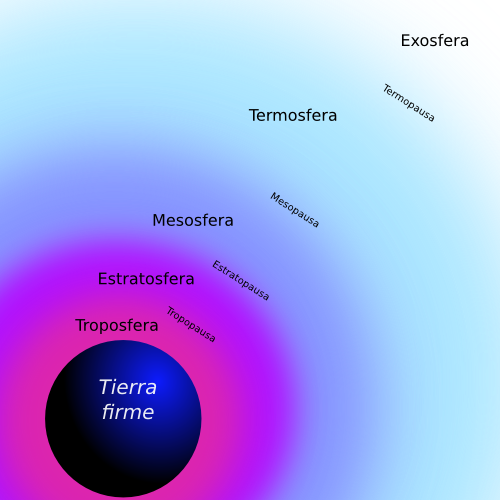
\includegraphics[scale=0.48]{Figures/CapasAtm}
\caption[Error por capas de la Atmósfera.]{Error por capas de la Atmósfera\footnotemark.}
\label{fig:ErrAtm}
\end{figure}

\footnotetext{Imagen tomada de: \href{https://upload.wikimedia.org/wikipedia/commons/0/03/Atmosferaterra.png}{https://upload.wikimedia.org/}}

Las señales de radio que comunican a los satélites y los receptores deben atravesar a la atmósfera a través de considerables kilómetros. El sólo hecho de atravesar partículas cargadas en la ionósfera\footnotemark y entrar en contacto con el vapor de agua de la tropósfera causa variaciones de velocidad en la transmisión. \\

El error en distancia atribuible a esta etapa es de 4 metros. 

\footnotetext{El error obtenido en la ionósfera puede eliminarse utilizando receptores de frecuencia doble L1 y L2.}

\subsubsection{Error causado por rutas múltiples}

\begin{figure}[!ht]
\centering
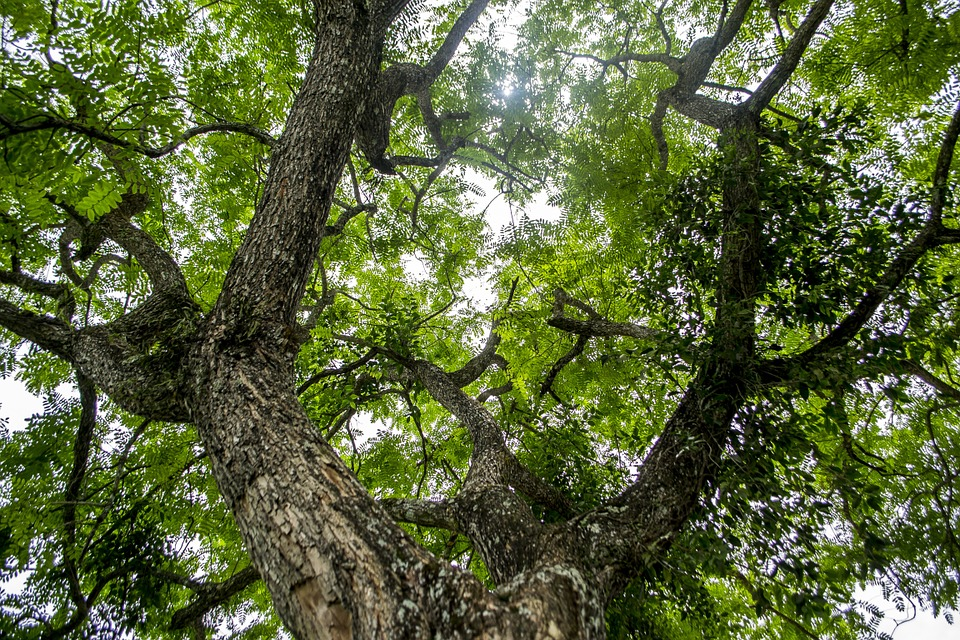
\includegraphics[scale=0.28]{Figures/RutasMult2}
\caption[Error por rutas múltiples.]{Error por rutas múltiples\footnotemark.}
\label{fig:ErrRMul}
\end{figure}

\footnotetext{Imagen tomada de: \href{https://pixabay.com/p-579199/?no_redirect}{https://pixabay.com/}}

 El sistema está diseñado para funcionar idealmente a cielo abierto. Sin embargo, en condiciones normales, esto no puede ser del todo reproducible, ya sea por el uso en áreas forestales o áreas urbanas. \\
 
Normalmente, la señal directa llega primero al receptor, y después, arriban las que proceden de las rutas múltiples. Esta diferencia de tiempo ocasiona otro error de medición. \\

Este mismo efecto era visible en las señales análogas de televisión, en las imágenes dobles. \\

Las nuevas antenas exteriores pueden filtrar este efecto.

\subsubsection{Error causado por el receptor}

Así como los satélites, los receptores cuentan con sus propios relojes. Debido a costos y dimensiones, éstos no pueden ser atómicos y por tanto son menos exactos, siendo otra fuente de error en la medición.\\

El error asociado a esta causa suele ser de 0.5 metros \cite{fallas2002sistema}.

\subsubsection{Error por Disponibilidad Selectiva}

\begin{figure}[!ht]
\centering

\includegraphics[scale=0.30]{Figures/RonaldReagan}
\caption[Presidente Ronald Reagan.]{Presidente Ronald Reagan\footnotemark.}
\label{fig:ErrDis}
\end{figure}

\footnotetext{Imagen tomada de: \href{https://www.goodfreephotos.com/albums/people/ronald-reagan-portrait-photo.jpg}{https://www.goodfreephotos.com/}}

GPS nació siendo un proyecto de tipo militar. Tras liberarse para uso civil en 1983 por autorización del presidente Ronald Reagan, se habilitaron dos secuencias codificadas llamadas códigos: C/A para uso civil y P para uso militar, con mayor precisión. \\

En el código C/A, se habilitó un error intencionado para evitar un alto grado de precisión, conocido como \textit{Disponibilidad Selectiva}. El presidente Bill Clinton ordenó eliminarle en el año 2000. de \cite{termal2014prototipo}.

GPS actualmente mantiene incorporada la opción de disponibilidad selectiva, cuyo error ronda los 100 metros, en caso de que el gobierno de Estados Unidos desee rehabilitarlo. \\

En 2007, el presidente de Estados Unidos anunción que los satélites de los bloques III no incorporarían más dicha opción \cite{chafer2017diseno}.

\section{Comunicación inalámbrica}

\begin{figure}[ht]
\centering

\includegraphics[scale=0.14]{Figures/wireless2}
\caption[Símbolo de conectividad inalámbrica.]{Símbolo de conectividad inalámbrica\footnotemark.}
\label{fig:ErrWrl}
\end{figure}

\footnotetext{Imagen tomada de: \href{https://pixabay.com/en/wireless-wi-fi-wireless-signal-1220904/}{https://pixabay.com/}}

Se dice que dos dispositivos se comunican de forma \textbf{inalámbrica} cuando éstos interactúan sin un contacto sólido entre sus masas. \\

En los aparatos electrónicos, se suelen usar ondas de radiofrecuencia, que a su vez se subclasifican dependiendo de la frecuencia a la que son emitidas.\\

A menor frecuencia, se obtiene una gran cobertura pero la capacidad se ve mermada. Conforme se aumenta la frecuencia, se pierde capacidad de cobertura pero la carga que puede tener una banda, aumenta. Se dice entonces que es una relación inversamente proporcional.\\

Actualmente no existe algún organismo internacional que regule las frecuencias utilizadas por los dispositivos de comunicación inalámbrica, por lo que cada país ha de adoptar una regulación propia. En Estados Unidos es la \textit{FCC} (Federal Communications Commission, Comisión Federal de Comunicaciones, por sus siglas en inglés) quien determina dichas regulaciones. Otras organizaciones reguladoras son la \textit{ISO} (International Organization for Standardization, Organización Internacional para la Estandarización, por sus siglas en inglés) y la \textit{EPCglobal}.

La clasificación del uso de las frecuencias por zona geográfica se muestra en la tabla \ref{Tab:BandasFreq}.

\begin{table}[!htb]
\begin{center}
\caption{Bandas de frecuencia en comunicación inalámbrica.}
\label{Tab:BandasFreq}
\begin{tabular}{|l|l|l|l|l|}
	\hline
	\textbf{País/Región} & \textbf{LF} & \textbf{HF} & \textbf{UHF} & \textbf{Microondas}\\
	\hline
	USA & 125-134 KHz & 13.56 MHz & 902-928 MHz & 2400-2483.5 MHz\\& & & & 5725-5850 MHz \\
	\hline
	Europa & 125-134 KHz & 13.56 MHz & 865-868 MHz & 2.45 GHz \\
	\hline
	Japón & 125-134 KHz & 13.56 MHz & No permitida & 2.45 GHz \\
	\hline
	China & 125-134 KHz & 13.56 MHz & No permitida & 2446-2454 MHz \\
	\hline
\end{tabular}
\end{center}
\end{table}

Tanto los sistemas LF y HF son para libre uso en todo el planeta. Sin embargo, UHF necesita de autorización y certificación dependiendo de la zona. En EUA, el uso de UHF no requiere de licencia, pero tiene algunas restricciones \cite{tapia2007identificacion}

\subsection{Protocolo ZigBee}

El estándar IEEE 802.15.4, mejor conocido como ZigBee, es una especificación para aplicaciones de control remoto para cualquier equipo que requiera de un bajo costo y un bajo consumo de potencia en entornos reducidos. ZigBee puede funcionar a tres bandas de frecuencia diferentes: 868 MHz, 915 MHz y 2.4 GHz. \\

\begin{figure}[ht]
\centering
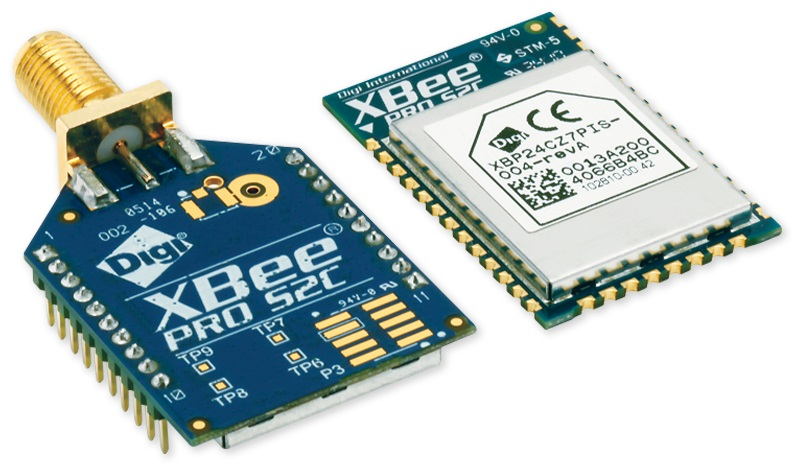
\includegraphics[scale=0.20]{Figures/xbee}
\caption[Equipo XBEE.]{Equipo XBEE\footnotemark.}
\label{fig:XBEE}
\end{figure}

\footnotetext{Imagen tomada de: \href{https://https://www.digi.com/products/xbee-rf-solutions/embedded-rf-modules-modems/xbee-zigbee/product-images/xbee-s2c-zigbee/}{https://www.digi.com/}}

Los módulos XBEE, fabricados por Digi International siguen el protocolo ZigBee. De entre todos esos módulos, destacan los de la serie PRO, ya que poseen una mayor potencia en la señal y en consecuencia, pueden hasta duplicar la capacidad de alcance en la distancia de transmisión. \\

El módulo requiere una alimentación que va desde los 2.8 V hasta los 3.4 V \cite{oyarce2010guia}.

\subsection{Módulo UHF del Ublox C94-M8P GPS}

Los dispositivos GPS Ublox C94-M8P están diseñados para trabajar en pares y vienen incorporados con módulos de comunicación inalámbrica que operan en los 915 MHz de frecuencia en el continente americano. \\

En él, se puede configurar el envío y recepción de diferentes contenidos. El manual de Ublox recomienda usar el formato RTCM3, que será explicado más adelante \citep{ubloxc94}.

\section{Sistemas de cómputo embebidos}

Los Sistemas Embebidos son sistemas programables, que realizan tareas específicas determinadas por el usuario, con el objetivo de optimizar los procesos para mejorar su desempeño y eficiencia, reduciendo tamaño y costos de producción. \\

Se caracterizan por el bajo consumo de energía. Está compuesto por tres componentes principales: Procesador, Dispositivos de almacenamiento y Periféricos \cite{caballero2014desarrollo}.

\subsection{BeagleBone Black}

\begin{figure}[ht]
\centering
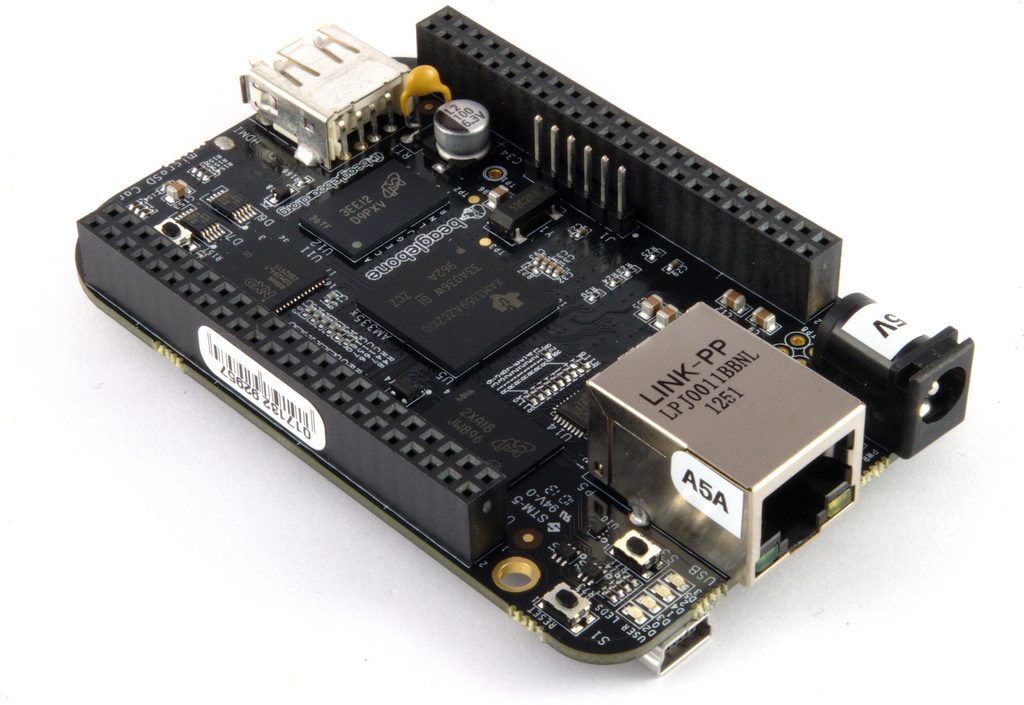
\includegraphics[scale=0.18]{Figures/BeagleBoneBlack}
\caption[BeagleBone Black.]{BeagleBone Black\footnotemark.}
\label{fig:BBlack}
\end{figure}

\footnotetext{Imagen tomada de: \href{https://www.flickr.com/photos/120586634@N05/14491195107}{https://www.flickr.com/}}

La BeagleBone es una plataforma de desarrollo de bajo costo. \\

Desarrollada por la BeagleBone Foundation de los Estados Unidos, una fundación sin ánimos de lucro, cuyo objetivo es la promoción de hardware y software de código abierto para el desarrollo de sistemas embebidos. \\

Por su diseño, posee una arquitectura ARM, que posee soporte de varias distribuciones Linux \cite{coronado2014desarrollo}. \\

Por su condición de hardware y software abierto, tanto sus esquemáticos del hardware, como las códigos fuente de su software están disponibles a todos los usuarios. \\

De las ventajas que posee una arquitectura como la del BeagleBone, basada en microprocesadores, es que su uso conduce a plataformas más poderosas, capaces de realizar tareas de gran carga computacional \cite{coley2013beaglebone}.

\section{Software Libre}
El \textbf{software} es un conjunto de instrucciones en lenguaje máquina para que una computadora realice funciones específicas.\\

El código máquina llega a través de un código más entendible para humanos, llamado código fuente, que un compilador se encarga de traducir a lenguaje máquina. Cuando el código fuente no es accesible para nadie, se dice que se trata de código cerrado \citep{i2005software}.\\

El software libre es aquél cuyo código fuente puede ser usado, copiado, estudiado, modificado y redistribuido libremente. A pesar de dicha capacidad de propagación del código, el software puede seguir siendo vendido comercialmente \citep{garcia2007promocion}. 

\subsection{GNU/Linux}
Linux es un sistema operativo. Un sistema operativo es un conjunto de programas que permiten la interacción con el hardware, además de ejecutar otros programas, así como crear una interfaz con el usuario. En un sistema GNU/Linux, Linux es el núcleo o kernel, y GNU es el conjunto de programas \citep{debian}. 


\section{Real Time Kinematics}

\begin{figure}[ht]
\centering
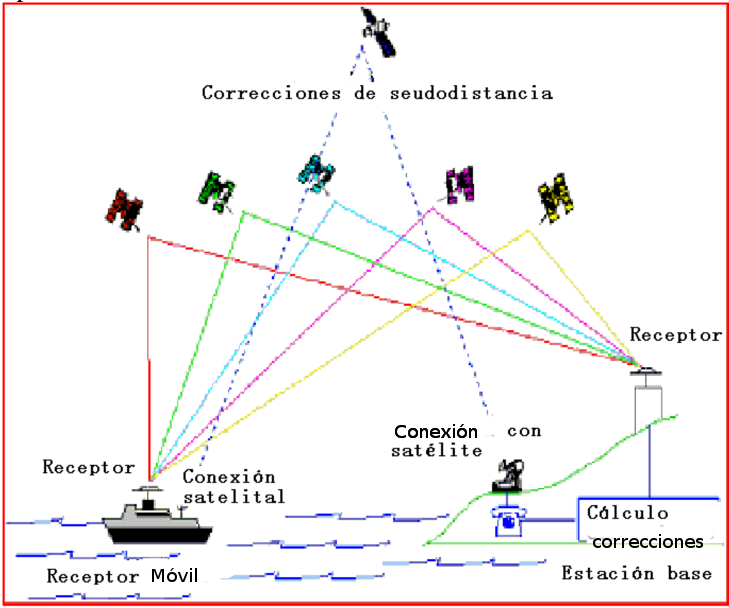
\includegraphics[scale=0.30]{Figures/DGPS1}
\caption[Esquema de funcionamiento en RTK.]{Esquema de funcionamiento en RTK, por \cite{fallas2002sistema}.}
\label{fig:RTK}
\end{figure}

Se le llama Sistema de Navegación Cinética Satelital en Tiempo Real (RTK, Real Time Kinematics por sus siglas en inglés), a las correcciones de la señal del GPS basadas en las señales L1 y L2. \\

Todo está en torno al siguiente supuesto: \\

Se tienen dos receptores a una distancia de pocos km entre sí. En esta condición, se podría esperar que los errores causados por el reloj atómico del satélite, por la ionósfera y la tropósfera afectarían de igual manera y con la misma magnitud a ambos receptores, por su proximidad. Si la posición exacta de uno de los receptores es conocida, entonces esta información puede ser usada para determinar el error asociado a las lecturas de dicho receptor y después aplicar la corrección al otro dispositivo. \\

Al GPS cuya posición es conocida recibe el nombre de \textbf{receptor base} y el segundo es llamado \textbf{receptor móvil}. La estación base calcula la distancia entre cada uno de los satélites de los que recibe señal y su posición (también conocida) para determinar el error asociado a la medición de distancia. Esa información la envía al receptor móvil, quien aplica la corrección hacia dicho satélite, obteniendo así un conocimiento más exacto sobre su posición \cite{fallas2002sistema}. \\

Con todas las correcciones aplicadas de forma ideal, se alcanza una precisión mejor a los 10 cm \cite{cerrato2011diseno}. \\

Conforme el receptor móvil se aleja gradualmente de la estación base, gradualmente, la utilidad de las correcciones proporcionadas de la segunda a la primera, disminuye \citep{mueller1994networked}.

\section{Formato RTCM-3}

Este formato es un estándar internacional para transmitir datos de posicionamiento en tiempo real. \\

Es utilizado sólo por las estaciones base para proporcionar sus observaciones. \\

Su estructura consiste en un mensaje de 42 bits fijos más otros bits que pueden variar de acuerdo al o los mensajes que se requiera enviar, como muestra la tabla \ref{Tab:RTCM-Struct}\cite{rubinov2011review}.\\

\begin{table}[!htb]
\begin{center}
\caption{Estructura del mensaje RTCM-3.}
\label{Tab:RTCM-Struct}
\begin{tabular}{|l|l|l|l|l|}
	\hline
	\textbf{Preámbulo} & \textbf{Reservado} & \textbf{\small Tamaño del mensaje} & \textbf{\small Datos del mensaje} & \textbf{Checksum}\\
	\hline
	8 bits & 6 bits & 10 bits & n bits & 24 bits \\
	\hline
	0xD3 & \parbox[t]{1.9cm}{Sin definir} & \parbox[t]{2.9cm}{Tamaño del mensaje en bytes} & \parbox[t]{2.9cm}{Tamaño variable en bytes} & \parbox[t]{2.05cm}{Definición QualComm CRC-24Q}\\
	\hline
\end{tabular}
\end{center}
\end{table}

El mensaje utilizado en este trabajo contendrá los siguientes datos: \\

\begin{table}[!htb]
\begin{center}
\caption{Contenido del mensaje en formato RTCM-3.1}
\begin{tabular}{|l|}
	\hline
	\textbf{Mensaje RTCM-3.1}\\
	\hline
	\tabitem \textbf{1005:} (X,Y,Z) Coordenadas fijas de la antena. \\
	\tabitem \textbf{1077:} Observaciones de GPS. \\
	\tabitem \textbf{1087:} Observaciones de GLONASS.\footnotemark \\
	\hline
\end{tabular}
\end{center}
\end{table}

\footnotetext{Homólogo ruso del sistema americano GPS.}

\section{RTKLIB}

Desarrollado por Tomoji Takasu, RTKLIB es un paquete de programas de código abierto escrito en C, para posicionamiento tanto estándar como preciso con sistemas de bajo costo. Soporta varios modos de posicionamiento tales como: Simple, Diferencial, Cinemático, entre otros. \\

En todos sus modos soporta tanto procesamiento en tiempo real así como postprocesamiento\cite{takasu2009development}.

\subsection{Modos de funcionamiento}

RTKLIB puede funcionar en distintos modos. Se explicarán un par de ellos en conformidad con su relevancia en este proyecto:

\begin{itemize}
\item Modo estático.
\item Modo cinemático.
\end{itemize}

RTKLIB utiliza un filtro de Kalman extendido (\textit{EKF}, extended Kalman filter, por sus siglas en inglés), para obtener los resultados de sus cálculos de aproximación. 

\subsubsection{Modo estático}
En este modo es necesaria una larga observación del cielo y de recolección de datos. Este requisito está fundamentado dado el cambio en la geometría del trayecto de los satélites, que apoyan en la resolución de ambigüedades\cite{wisniewski2013evaluation}.

\subsubsection{Modo cinemático}
Requerido cuando el objeto al que se quiere conocer su posición, se encuentra en movimiento. Permite obtener decímetros de precisión. Para un funcionamiento óptimo, necesita las coordenadas de una estación base conocida en el archivo de configuración. Los datos de esta estación fija pueden ser obtenidos mediante mensajes RTCM\cite{wisniewski2013evaluation}.

\section{Vehículos aéreos no tripulados - VANT}

\begin{figure}[ht]
\centering
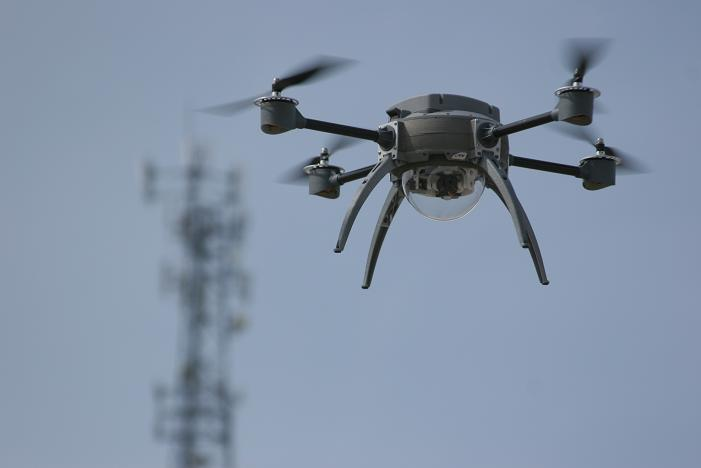
\includegraphics[scale=0.30]{Figures/UAV}
\caption[Vehículo aéreo no tripulado.]{Vehículo aéreo no tripulado\footnotemark.}
\label{fig:UAV}
\end{figure}

\footnotetext{Imagen tomada de \href{https://upload.wikimedia.org/wikipedia/commons/7/79/Aeryon_Scout_In_Flight.jpg}{https://upload.wikimedia.org/}}

Los vehículos aéreos no tripulados (\textit{VANT} o \textit{UAV}, Unmanned Aerial Vehicle por sus siglas en inglés) estuvieron orientados inicialmente para operaciones de contexto militar \citep{fahlstrom2012introduction}.\\

Un VANT es definido como un vehículo con operaciones y sistemas mecatrónicos, con computadoras a bordo y supervisado por humanos desde tierra \citep{haluani2015tecnologia}.\\

En usos civiles, se pueden destacar empresas que investigan formas de entregar paquetes mediante el uso de esta tecnología, así como observaciones meteorológicas.\\

Algunas áreas de aplicación son \citep{addati2014introduccion}:

\begin{itemize}
\item Imágenes y vídeo aéreo.
\item Monitoreo y vigilancia.
\item Inspección de infraestructuras.
\item Búsqueda y rescate.
\item Gestión de emergencias.
\item Mapeo de terrenos.
\end{itemize}

\subsection{Instrumentación de vuelo}

La instrumentación de vuelo es la encargada de obtener el estado de vuelo del UAV de manera precisa, así como el entorno en el que se encuentra haciendo uso de distintos sensores.\\

Dependiendo de la finalidad de una misión de vuelo, se pueden encontrar los siguientes sistemas de sensado \citep{barrientos2007vehiculos}:\\

Para un marco de referencia inercial.
\begin{itemize}
\item Acelerómetros.
\item Giroscopios.
\end{itemize}
Para posicionamiento y velocidad.
\begin{itemize}
\item GPS.
\item Compás.
\end{itemize}

\section{Conclusión}

Tras una revisión de los conceptos y componentes necesarios, se procede a continuación a detallar la forma en cómo cada uno de ellos conforma un elemento clave para la obtención del objetivo.\\

En el capítulo \ref{Chap:DisHard}, se habla acerca de la integración de los componentes descritos en el capítulo \ref{Chap:Marco}. Se presentan descripciones acerca de los componentes, fotografías, especificaciones de funcionamiento y modos de operación, así como las condiciones de uso para un correcto desempeño. 